% A Readymade beamer presentation template
% Version 1.1
% Relase date: May 2, 2010
% Released at http://www.stattler.com
% by Rifat Jahan

\documentclass{beamer}
%\usecolortheme[named=green]{structure}
\mode<presentation> {
\usetheme{Madrid} % My favorite!
%\usetheme{Boadilla} % Pretty neat, soft color.
%\usetheme{default}
%\usetheme{Warsaw}
%\usetheme{Bergen} % This template has nagivation on the left
%\usetheme{Frankfurt} % Similar to the default with an extra region at the top.
%\usecolortheme{seahorse} % Simple and clean template
%\usetheme{Darmstadt} % not so good
% Uncomment the following line if you want page numbers and using Warsaw theme
% \setbeamertemplate{footline}[page number]
%\setbeamercovered{transparent}
\setbeamercovered{invisible}
% To remove the navigation symbols from the bottom of slides%
\setbeamertemplate{navigation symbols}{} 
}

\usepackage{graphicx}
%\usepackage{bm} 
% For typesetting bold math (not \mathbold)
%\logo{\includegraphics[height=0.6cm]{yourlogo.eps}}

\title[Subspaces]{Face Recognition in Subspaces}

\author{Josh Klontz}
%\institute[U of X]
%{
%University of [...] \\
%\medskip
%{\emph{email@domain.ca}}
%}
\date{\today}
% \today will show current date. 
% Alternatively, you can specify a date.

\begin{document}

\begin{frame}
\titlepage
\end{frame}

\section{Introdution}
\begin{frame}
\frametitle{Works Covered}
\begin{block}{Bayesian face recognition}
Moghaddam, Baback, Tony Jebara, and Alex Pentland. "Bayesian face recognition." Pattern Recognition 33.11 (2000): 1771-1782.
\end{block}
\pause
\begin{block}{Probabilistic models for inference about identity}
Li, Peng, et al. "Probabilistic models for inference about identity." Pattern Analysis and Machine Intelligence, IEEE Transactions on 34.1 (2012): 144-157.
\end{block}
\pause
\begin{block}{Bayesian Face Revisited: A Joint Formulation}
Chen, Dong, et al. "Bayesian Face Revisited: A Joint Formulation."
\end{block}
\end{frame}

\section{Bayesian face recognition}
\begin{frame}
\frametitle{Bayesian face recognition}
\begin{block}{Abstract}
\begin{itemize}
\item \emph{Probabilistic} measure of similarity.
\pause
\item Replace costly \emph{nonlinear} (on-line) computation of Bayesian similarity measure with inexpensive \emph{linear} (off-line) subspace projections and Euclidean norms.
\pause
\item Top performer in 1996 \emph{FERET} face recognition competition.
\end{itemize}
\end{block}
\end{frame}

\begin{frame}
\frametitle{A Bayesian approach}
\begin{block}{Previous Work}
Rely on similarity metrics based on Euclidean distance or normalized correlation.
\pause
Also known as:
\begin{itemize}
\item Template matching
\item Nearest-neighbor-based recognition
\end{itemize}
\end{block}
\pause
\begin{block}{Proposed Approach}
\emph{Probabilistic} similarity measure
\pause
\begin{align}
\Delta& = I_1 - I_2 \\
\Omega_I& \equiv \text{Intrapersonal variations (\emph{same} individual)} \\
\Omega_E& \equiv \text{Extrapersonal variations (\emph{different} individuals)} \\
S(I_1,I_2)& = P(\Delta \in \Omega_I) = P(\Omega_I | \Delta)
\end{align}
\end{block}
\end{frame}

\begin{frame}
\frametitle{Probabilistic similarity measures}
\begin{block}{Bayes Rule}
\begin{equation}
\begin{split}
S(I_1,I_2)& = P(\Omega_I | \Delta) \\
& = \frac{P(\Delta|\Omega_I)P(\Omega_I)}{P(\Delta|\Omega_I)P(\Omega_I)+P(\Delta|\Omega_E)P(\Omega_E)}\equiv \text{MAP} \\
& \approx P(\Delta|\Omega_I)\equiv \text{ML}
\end{split}
\end{equation}
\end{block}
\pause
\begin{block}{Learning Problem}
\begin{itemize}
\item Estimate $P(\Delta|\Omega_I)$ and $P(\Delta|\Omega_E)$ from training data.
\pause
\item Assume both classes are Gaussian-distributed.
\pause
\item \emph{Note:} Bayesian formulation casts the standard face recognition task (essentially an $M$-ary classification problem for $M$ individuals) into a \emph{binary} pattern classification problem with $\Omega_I$ and $\Omega_E$.
\end{itemize}
\end{block}
\end{frame}

\begin{frame}
\frametitle{Subspace density estimation}
\begin{block}{Observations}
\begin{itemize}
\item Intensity difference vector is very high-dimensional: $\Delta \in \mathbb{R}^N \approx O(10^4)$.
\pause
\item Insufficient training examples to compute second-order statistics.
\pause
\item Formidable computational cost even if it was possible.
\pause
\item \emph{Intrinsic} dimensionality of $\Delta$ likely to be significantly smaller.
\end{itemize}
\end{block}
\pause
\begin{block}{Solution}
Approximate $\Delta$ in a lower dimensional PCA subspace: $\Delta^\prime \in \mathbb{R}^M$ such that $M << N$.
\end{block}
\end{frame}

\begin{frame}
\frametitle{Subspace Projection}
\begin{figure}[H]
\centering
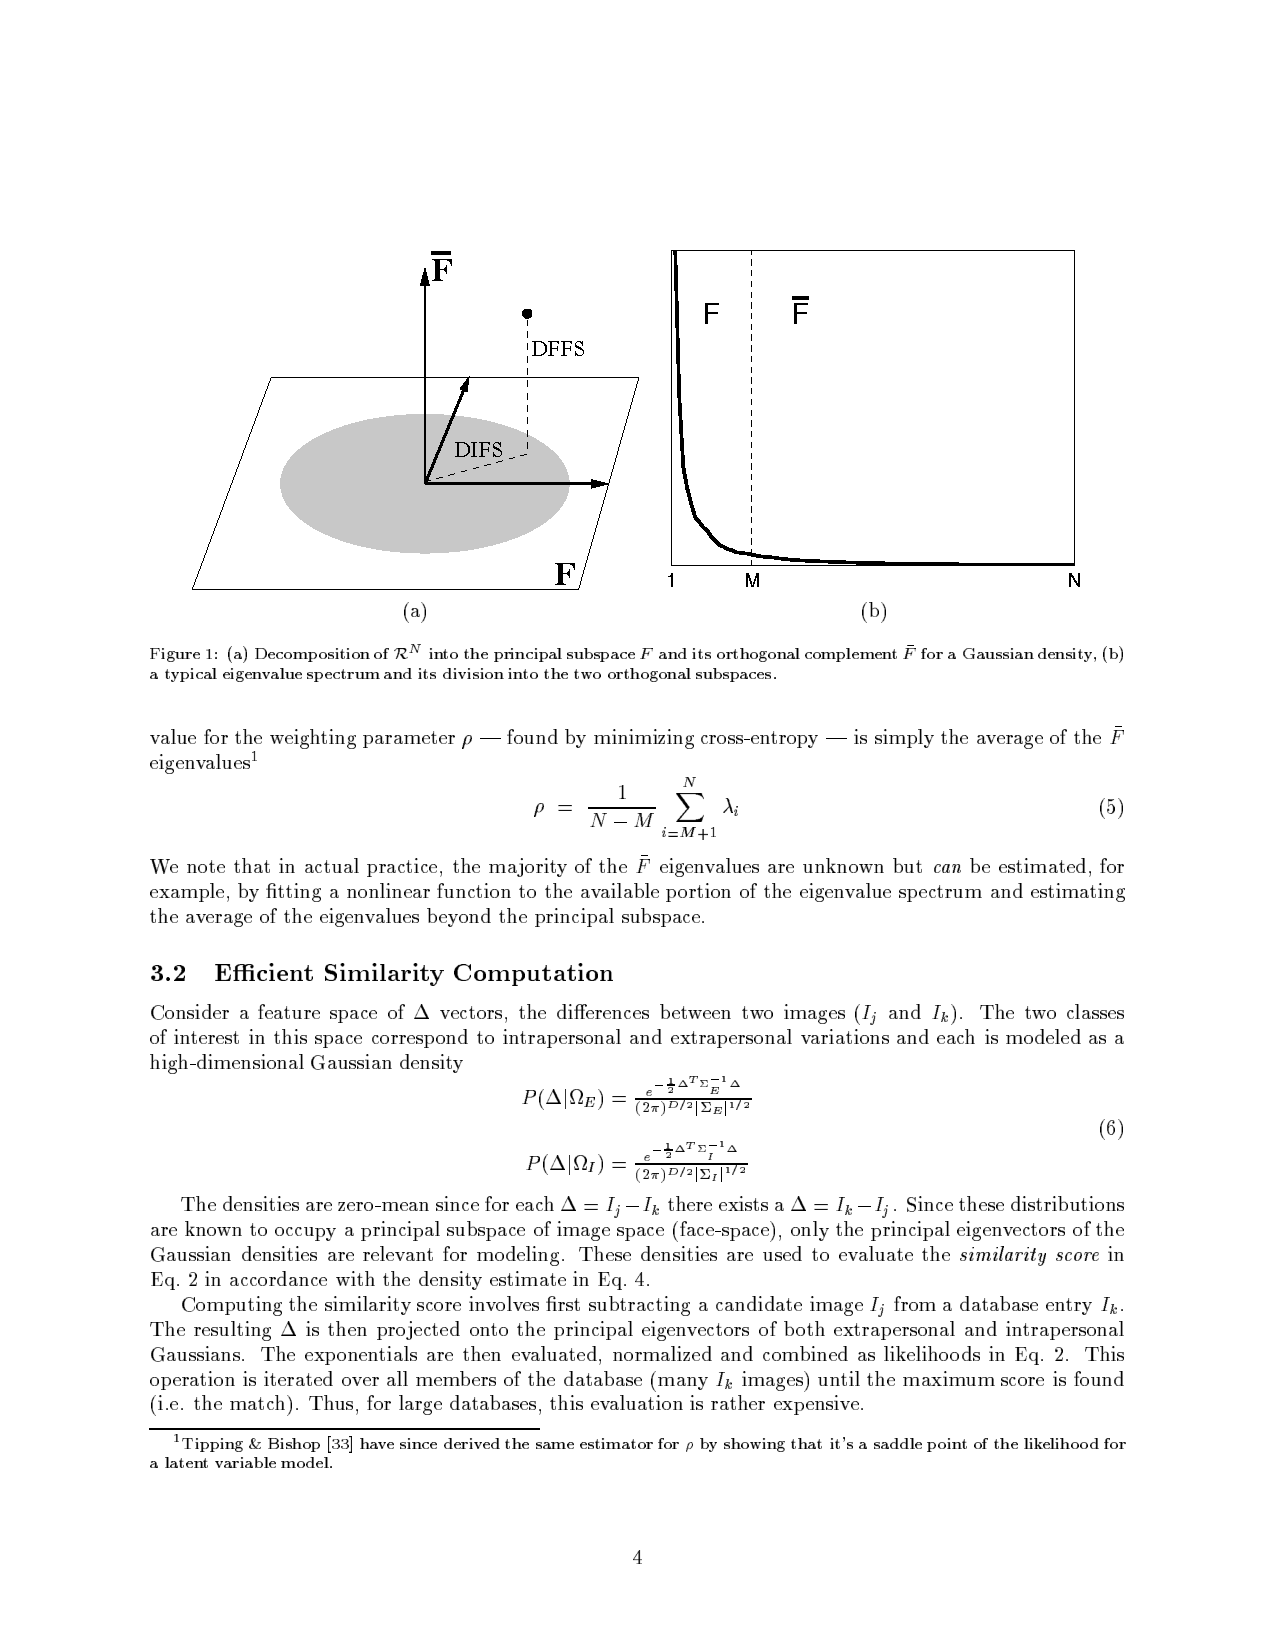
\includegraphics[width=\textwidth, trim=1in 6.4in 1in 1.6in, clip]{Moghaddam6}
\end{figure}
\end{frame}

\begin{frame}
\frametitle{Subspace density estimation}
\begin{block}{Solution details}
Learn subspaces for both $P(\Delta|\Omega_I)$ and $P(\Delta|\Omega_E)$.
\pause
Then approximate $P(\Delta|\Omega)$ with the following observation:
\begin{equation}
\begin{split}
P(\Delta|\Omega)& = P_f(\Delta|\Omega)P_{\bar{f}}(\Delta|\Omega) \\
& \approx P_f(\Delta|\Omega)\hat{P}_{\bar{f}}(\Delta|\Omega) \\
& = \left[\exp\frac{-\frac{1}{2}\sum_{i=1}^My_i^2/\lambda_i}{(2\pi)^{M/2}\prod_{i=1}^M\lambda_i^{1/2}}\right]\left[\frac{\exp(-\epsilon^2(\Delta)/2p)}{(2\pi p)^{(N-M)/2}}\right] \\
\end{split}
\end{equation}
\pause
where
\begin{align}
\epsilon^2(\Delta)& = \text{Residual Reconstruction Error} = \text{DFFS} \\
p& = \frac{1}{N-M}\sum_{i=M+1}^N\lambda_i
\end{align}
\end{block}
\end{frame}

\begin{frame}
\frametitle{Visualization}
\begin{figure}[H]
\centering
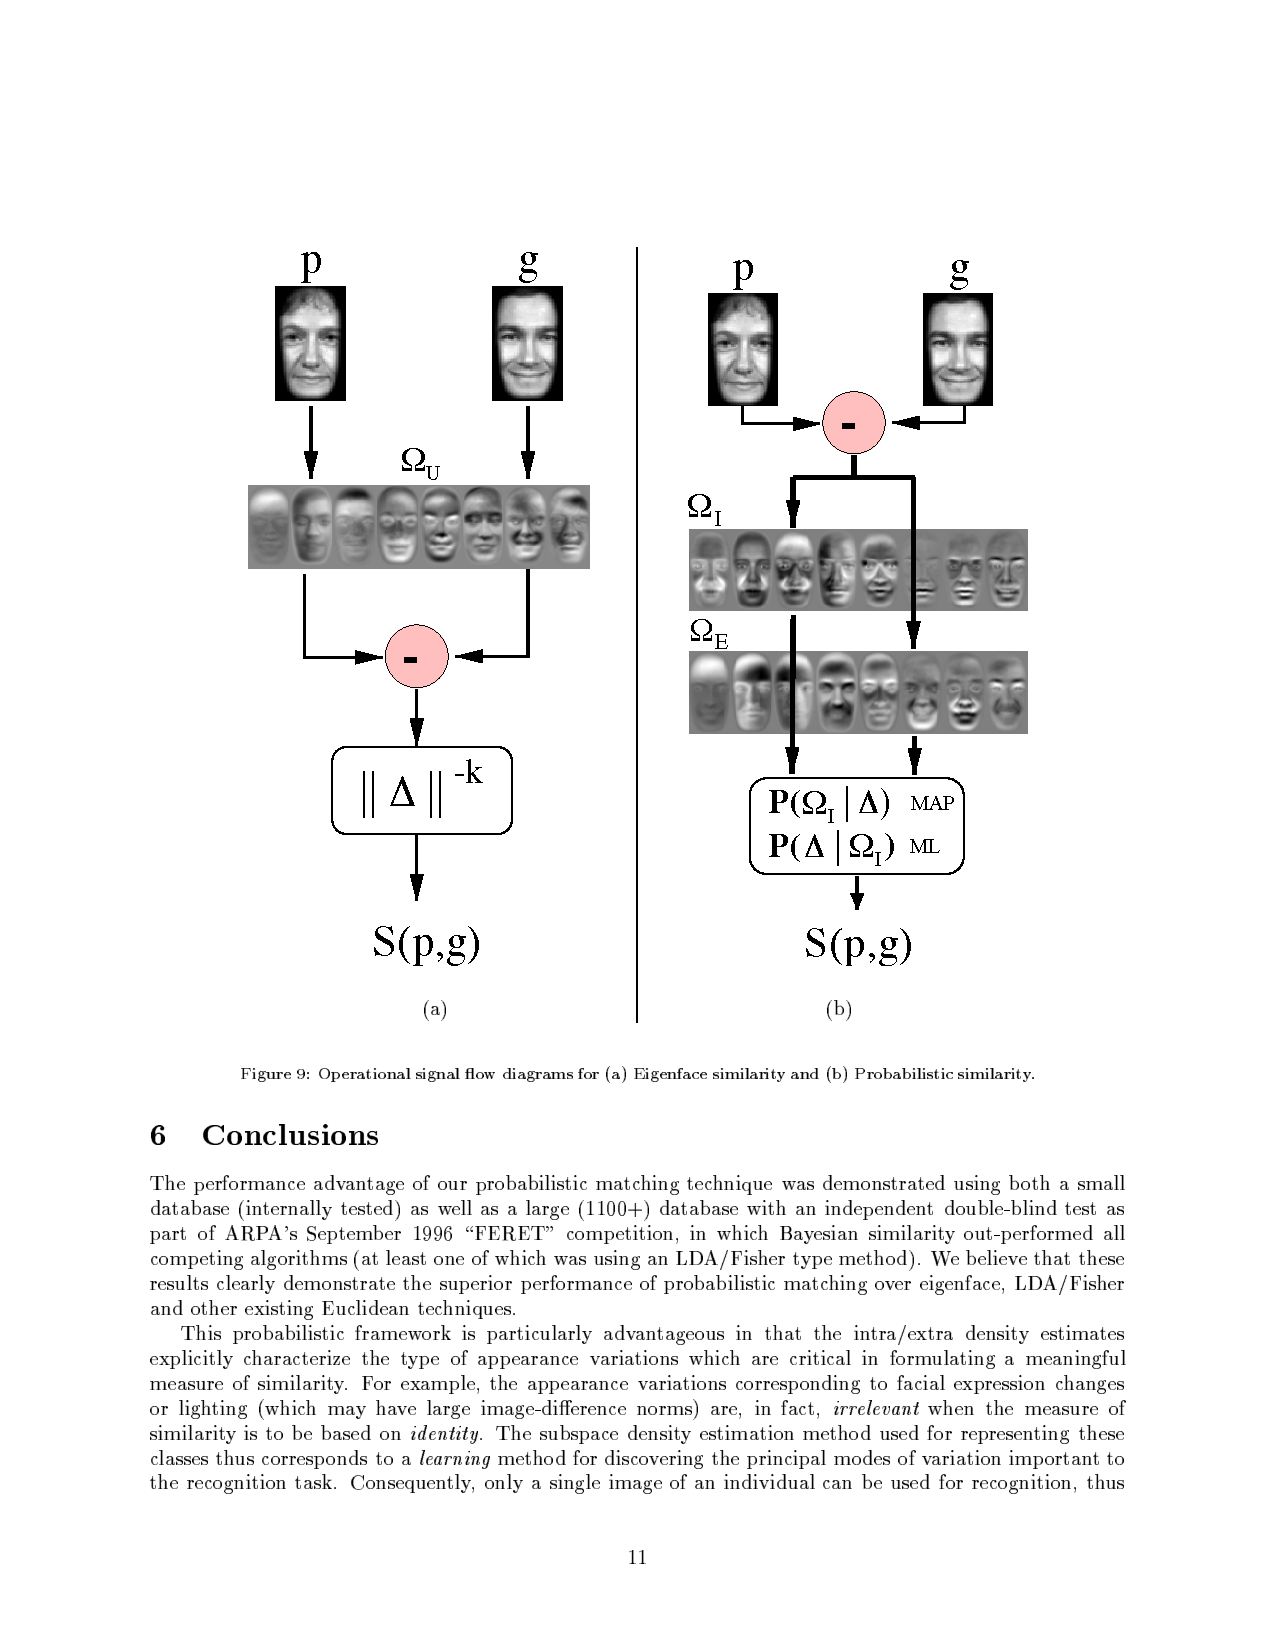
\includegraphics[height=\textheight, trim=1.6in 3.75in 1.6in 1.6in, clip]{Moghaddam13}
\end{figure}
\end{frame}

\begin{frame}
\frametitle{Efficient similarity computation}
\begin{block}{The Problem}
Expensive similarity computation
\begin{itemize}
\pause
\item Subtract the candidate image $I_j$ from the database entry $I_k$.
\pause
\item Project the resulting $\Delta$ onto the principal eigenvectors of both the extrapersonal and intrapersonal Gaussians.
\pause
\item Evaluate the exponentials are plug into Bayes formula.
\pause
\item Repeat for all images in the database
\end{itemize}
\end{block}
\end{frame}

\begin{frame}
\frametitle{Efficient similarity computation}
\begin{block}{The Solution}
Pre-process each image with \emph{whitening} transformations, representing the image as two vectors of whitened subspace coefficients
\pause
\begin{equation}
\mathbf{i}_j=\Lambda_I^{-1/2}V_II_j\ \ \ \ \mathbf{e}_j=\Lambda_E^{-1/2}V_EI_j
\end{equation}
\pause
and evaluating likelihoods is reduced to computing Euclidean distances
\begin{equation}
\begin{split}
P(\Delta|\Omega_E)& = \frac{e^{-1/2}||\mathbf{e_j}-\mathbf{e_k}||^2}{(2\pi)^{D/2}|\Sigma_E|^{1/2}} \\
P(\Delta|\Omega_I)& = \frac{e^{-1/2}||\mathbf{i_j}-\mathbf{i_k}||^2}{(2\pi)^{D/2}|\Sigma_I|^{1/2}}
\end{split}
\end{equation}
\end{block}
\pause
\begin{block}{Question}
What happened to $\hat{P}_{\bar{f}}(\Delta|\Omega)$, $\epsilon^2(\Delta)$, and $p$?
\end{block}
\end{frame}

\begin{frame}
\frametitle{``Dual'' Eigenfaces}
\begin{figure}[H]
\centering
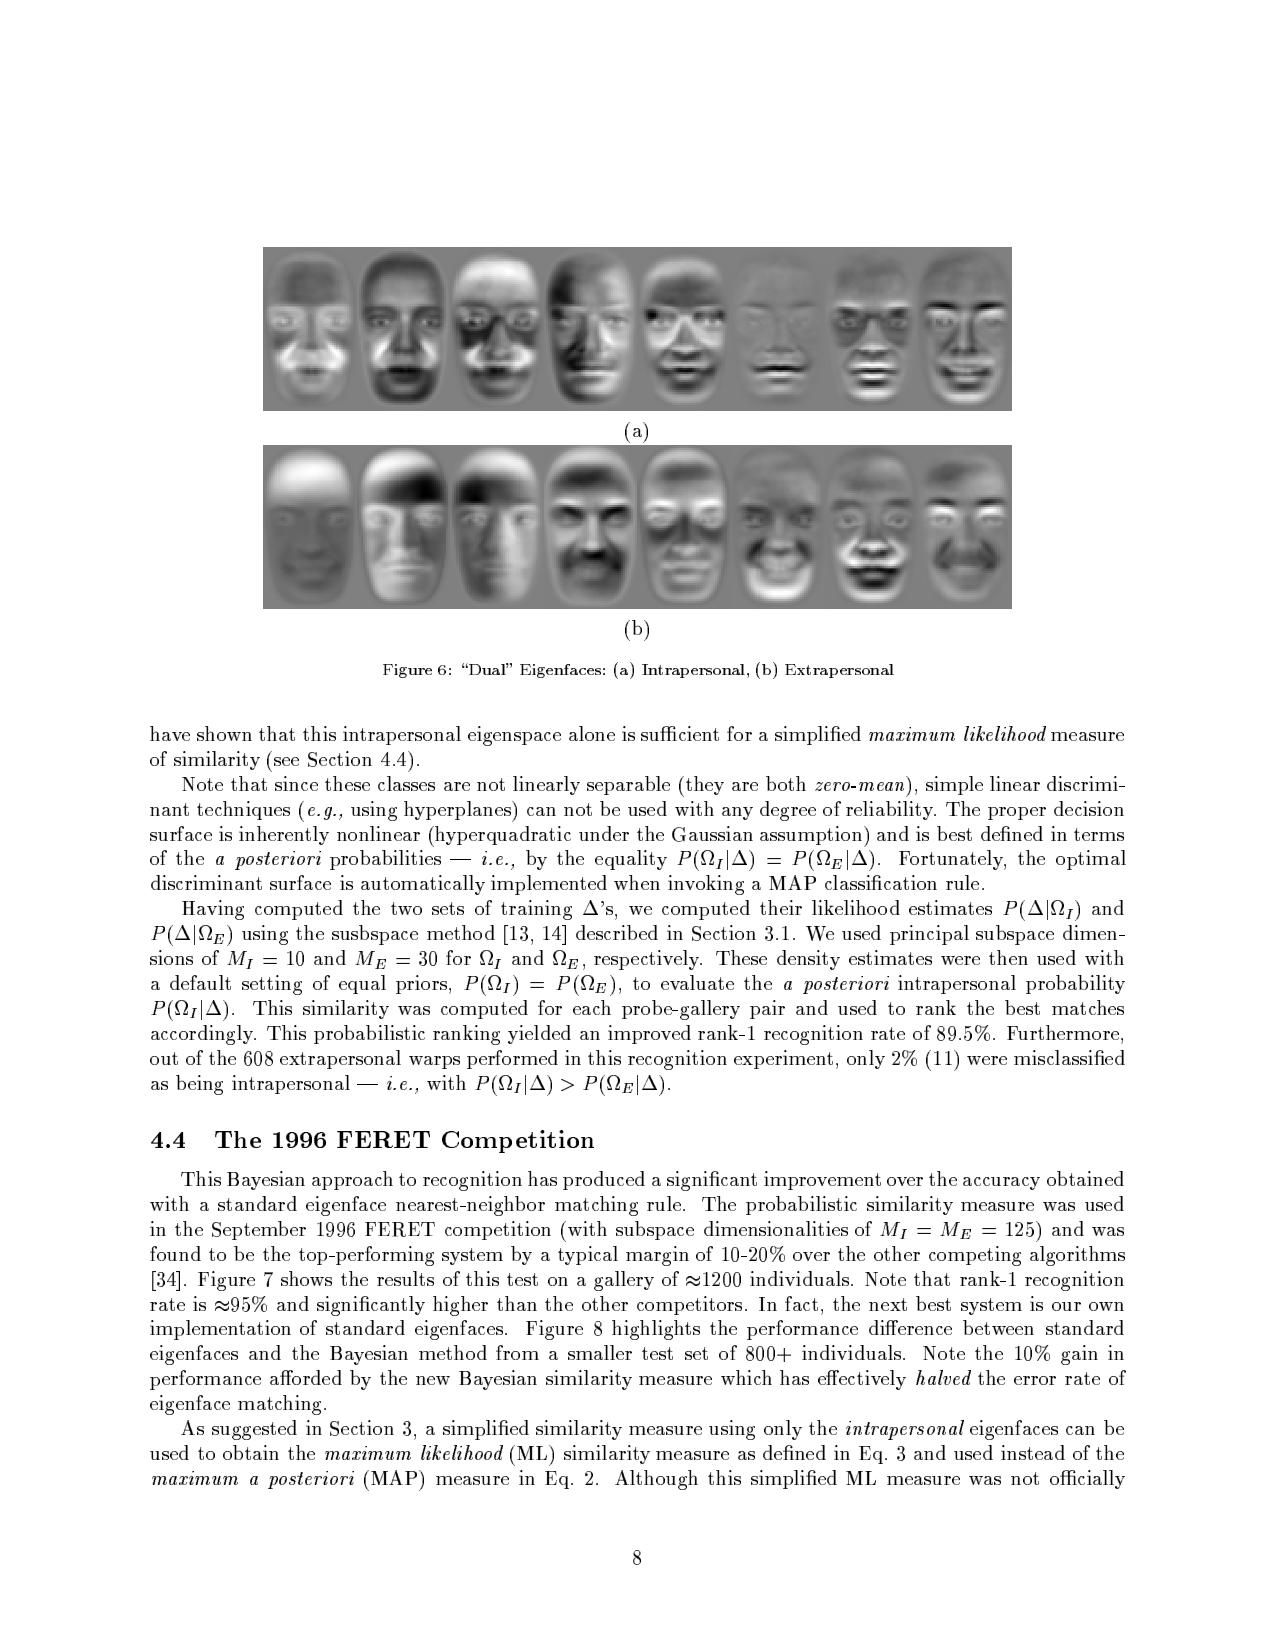
\includegraphics[width=\textwidth, trim=1.6in 6.4in 1.6in 1.6in, clip]{Moghaddam10}
\end{figure}
\end{frame}

\begin{frame}
\frametitle{Results}
\begin{figure}[H]
\centering
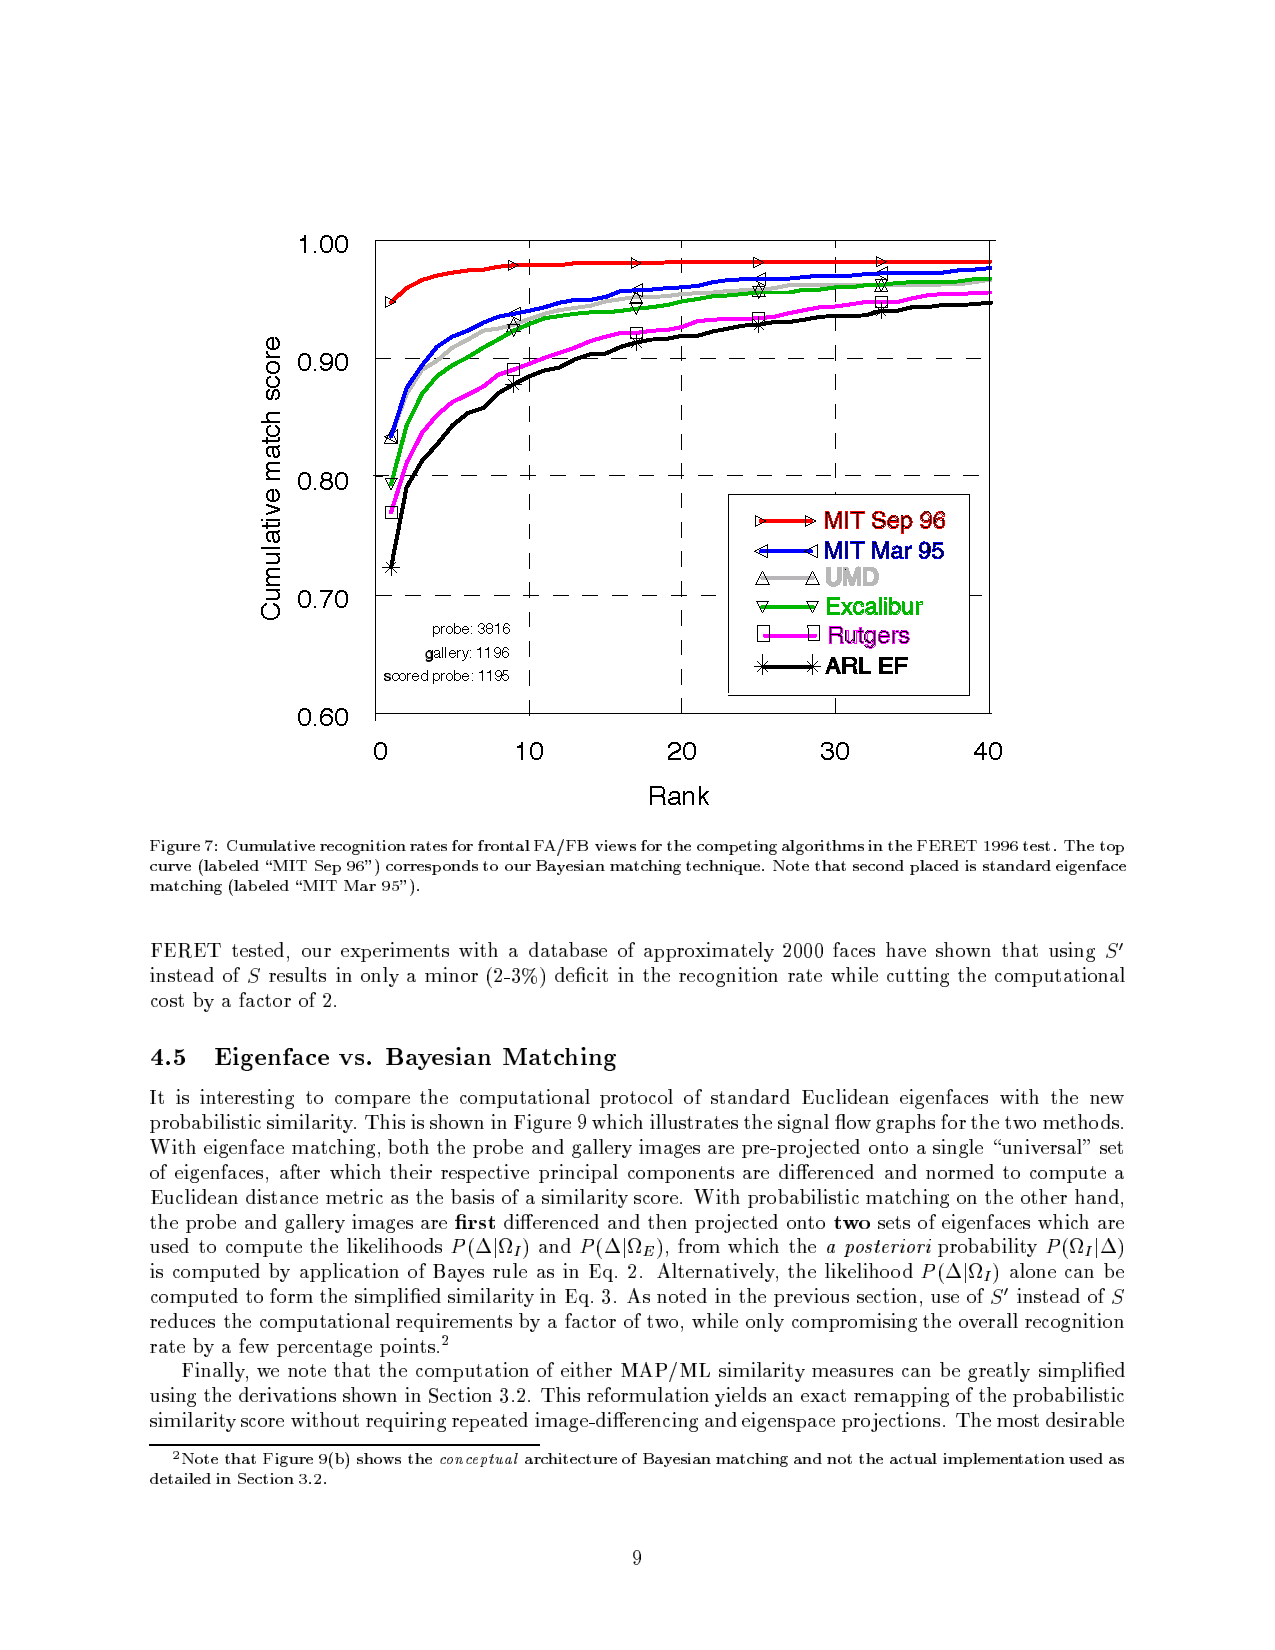
\includegraphics[height=\textheight, trim=1.6in 4.9in 1.6in 1.4in, clip]{Moghaddam11}
\end{figure}
\end{frame}

\begin{frame}
\centerline{The End!}
\end{frame}

% End of slides
\end{document}